
%%%%%%%% ICML 2018 EXAMPLE LATEX SUBMISSION FILE %%%%%%%%%%%%%%%%%

\documentclass{article}

% Recommended, but optional, packages for figures and better typesetting:
\usepackage{microtype}
\usepackage{graphicx}
\usepackage{subfigure}
\usepackage{booktabs} % for professional tables

% hyperref makes hyperlinks in the resulting PDF.
% If your build breaks (sometimes temporarily if a hyperlink spans a page)
% please comment out the following usepackage line and replace
% \usepackage{icml2018} with \usepackage[nohyperref]{icml2018} above.
\usepackage{hyperref}

% Attempt to make hyperref and algorithmic work together better:
\newcommand{\theHalgorithm}{\arabic{algorithm}}

\newcommand{\system}{\textsc{HelmholtzHacker}~}

% Use the following line for the initial blind version submitted for review:
\usepackage{icml2018}


\usepackage{hyperref}       % hyperlinks
\usepackage{url}            % simple URL typesetting
\usepackage{booktabs}       % professional-quality tables
\usepackage{amsfonts}       % blackboard math symbols
\usepackage{nicefrac}       % compact symbols for 1/2, etc.
\usepackage{microtype}      % microtypography

\usepackage{listings}
\usepackage{amsthm}
% use Times
\usepackage{times}
% For figures
\usepackage{graphicx} % more modern
%\usepackage{epsfig} % less modern
\usepackage{subfig} 
\usepackage{fancyvrb}


\usepackage{caption}
\usepackage{subcaption}

\fvset{fontsize=\footnotesize}

\usepackage{amssymb}
\usepackage{listings}
\usepackage{wrapfig}
\usepackage{tabularx}


\usepackage{verbatim}
 \usepackage{booktabs}
 % For algorithms
\usepackage{algorithm}
\usepackage{algorithmic}
\usepackage{tikz}
\usetikzlibrary{fit,bayesnet}
%\usetikzlibrary{arrows.meta}
%\usetikzlibrary{positioning}
%\usetikzlibrary{decorations.text}
%\usetikzlibrary{decorations.pathmorphing}
\usepackage{dsfont}
\usepackage{amsmath}
\usepackage{hyperref}
\DeclareMathOperator*{\argmin}{arg\,min} % thin space, limits underneath in displays
\DeclareMathOperator*{\argmax}{arg\,max} % thin space, limits underneath in displays
\DeclareMathOperator{\argmin}{argmin} % no space, limits underneath in displays



% Packages hyperref and algorithmic misbehave sometimes.  We can fix
% this with the following command.

\newcommand{\Expect}{\mathds{E}} %{{\rm I\kern-.3em E}}
\newcommand{\indicator}{\mathds{1}} %{{\rm I\kern-.3em E}}
\newcommand{\expect}{\mathds{E}} %{{\rm I\kern-.3em E}}
\newcommand{\probability}{\mathds{P}} %{{\rm I\kern-.3em P}}



% If accepted, instead use the following line for the camera-ready submission:
%\usepackage[accepted]{icml2018}

% The \icmltitle you define below is probably too long as a header.
% Therefore, a short form for the running title is supplied here:
\icmltitlerunning{Inducing Domain Specific Languages for Bayesian Program Learning}

\begin{document}

\twocolumn[
\icmltitle{Inducing Domain Specific Languages for Bayesian Program Learning}

% It is OKAY to include author information, even for blind
% submissions: the style file will automatically remove it for you
% unless you've provided the [accepted] option to the icml2018
% package.

% List of affiliations: The first argument should be a (short)
% identifier you will use later to specify author affiliations
% Academic affiliations should list Department, University, City, Region, Country
% Industry affiliations should list Company, City, Region, Country

% You can specify symbols, otherwise they are numbered in order.
% Ideally, you should not use this facility. Affiliations will be numbered
% in order of appearance and this is the preferred way.
\icmlsetsymbol{equal}{*}

\begin{icmlauthorlist}
\icmlauthor{Aeiau Zzzz}{equal,to}
\icmlauthor{Bauiu C.~Yyyy}{equal,to,goo}
\icmlauthor{Cieua Vvvvv}{goo}
\icmlauthor{Iaesut Saoeu}{ed}
\icmlauthor{Fiuea Rrrr}{to}
\icmlauthor{Tateu H.~Yasehe}{ed,to,goo}
\icmlauthor{Aaoeu Iasoh}{goo}
\icmlauthor{Buiui Eueu}{ed}
\icmlauthor{Aeuia Zzzz}{ed}
\icmlauthor{Bieea C.~Yyyy}{to,goo}
\icmlauthor{Teoau Xxxx}{ed}
\icmlauthor{Eee Pppp}{ed}
\end{icmlauthorlist}

\icmlaffiliation{to}{Department of Computation, University of Torontoland, Torontoland, Canada}
\icmlaffiliation{goo}{Googol ShallowMind, New London, Michigan, USA}
\icmlaffiliation{ed}{School of Computation, University of Edenborrow, Edenborrow, United Kingdom}

\icmlcorrespondingauthor{Cieua Vvvvv}{c.vvvvv@googol.com}
\icmlcorrespondingauthor{Eee Pppp}{ep@eden.co.uk}

% You may provide any keywords that you
% find helpful for describing your paper; these are used to populate
% the "keywords" metadata in the PDF but will not be shown in the document
\icmlkeywords{Machine Learning, ICML}

\vskip 0.3in
]

% this must go after the closing bracket ] following \twocolumn[ ...

% This command actually creates the footnote in the first column
% listing the affiliations and the copyright notice.
% The command takes one argument, which is text to display at the start of the footnote.
% The \icmlEqualContribution command is standard text for equal contribution.
% Remove it (just {}) if you do not need this facility.

%\printAffiliationsAndNotice{}  % leave blank if no need to mention equal contribution
\printAffiliationsAndNotice{\icmlEqualContribution} % otherwise use the standard text.

\begin{abstract}
This document provides a basic paper template and submission guidelines.
Abstracts must be a single paragraph, ideally between 4--6 sentences long.
Gross violations will trigger corrections at the camera-ready phase.
\end{abstract}

\section{Introduction}

Automatically inducing programs from examples is a long-standing goal
of artificial intelligence.  Recent work in program induction show
that deep networks can be very successful at learning to write certain
kinds of programs (e.g., RobustFill:~\cite{devlin2017robustfill} and
DeepCoder:~\cite{balog2016deepcoder}), as can symbolic search
techniques (e.g., Metagol:~\cite{muggleton2015meta} and 
FlashFill:~\cite{gulwani2011automating}).
However, the success of these approaches -- both symbolic and neural --
relies crucially upon a hand-engineered \emph{Domain Specific Language} (DSL).
The DSL is an inventory of restricted programming primitives,
that imparts domain specific knowledge about the space of programs.
To what extent can we dispense with hand-engineered DSLs?

This work proposes \emph{learning} DSLs.
We consider the problem of solving many related program induction tasks,
starting with a Lisp-like representation.
We introduce an algorithm, called the \system,
which creates its own DSL by discovering and then reusing
new useful programming idioms and subroutines.





%% Imagine an agent faced with a new domain of unfamiliar tasks: think
%% playing new kinds of videogames, authoring Python code, or navigating
%% through mazes.  Our agent has at its disposal a basis of primitive
%% actions it can compose to propose solutions to these tasks, but it is
%% no idea what kinds of primitives are appropriate for which tasks
%% nor does it know the higher-level vocabulary in which solutions are
%% best expressed.  How can our agent learn to solve problems in this new
%% domain?


%% The AI and machine learning literature contains two broad takes on this problem.
%% The first take is that the agent should come up with a better representation of the space of solutions,
%% for example, by inventing new primitive actions: see \emph{options} in reinforcement learning~\cite{stolle2002learning}, the EC algorithm in program synthesis~\cite{Dechter:2013:BLV:2540128.2540316}, or predicate invention in inductive logic programming~\cite{muggleton2015meta}.
%% The second take is that the agent should learn a discriminative model mapping problems to a distribution over solutions: for example, policy gradient methods in reinforcement learning or neural models of program synthesis~\cite{devlin2017robustfill,balog2016deepcoder}.
%% Our contribution is a general algorithm for fusing these two takes on the problem:
%% we propose jointly inducing a representation language, called a \emph{Domain Specific Language} (DSL),
%% alongside a bottom-up discriminative model that regresses from problems to solutions.
%% We evaluate our algorithm on four domains:
%% building Boolean circuits; symbolic regression; FlashFill-style~\cite{gulwani2011automating} string processing problems; and functions on lists.
%% %Because we want a domain-general
%% %approach,
%% We model solutions to tasks as
%% programs,
%% which frames our problem as one of program induction.

\begin{figure}
  \centering

  \begin{tikzpicture}

  \node[latent] at (0.5,3) (d){$\mathcal{D}$};
  \node[latent] at (1.5,3) (t){$\theta$};
  \node[latent] at (1,1.75) (z){$p$};
%  \node[latent] at (3.5,1.5) (tx){$\theta^{(x)}$};
  \node[obs] at (1,0) (x) {$x$};
  \edge {z}{x};
  \edge {d,t}{z};
  \plate {}{(z)(x)}{$x\in X$};
  \node[align = center] at ([yshift = -1.3cm]x.south) {(a) \\generative \\model};

  \begin{scope}[shift = {(-1,0)}]  
  \node[latent] at (3.5,3) (dx){$\mathcal{D}$};
  \node[latent] at (3.5,1.75) (zp){$p$};
  \node[latent] at (5.5,1.75) (tx){$\theta^{(x)}$};
  \node[obs] at (3.5,0) (xp) {$x$};
  \plate {}{(zp)(xp)(tx)}{$x\in X$};
  \node[align = center] at ([yshift = -1.2cm,xshift = 1cm]xp.south) {(b) \\recognition model};
  \draw [->,red] (xp.east) to[out = 0,in = -90] node(nn){} (tx.south);
  \draw [->,red] (tx.west) -- (zp.east);
  \draw [->,red] (dx.south) -- (zp.north);

  \node at (nn) {
    \begin{tikzpicture}[x=2.5cm,y=1.25cm,transform canvas={scale=0.2,shift={+(-1,2.5)}}]
      \tikzstyle{neuron}=[circle,fill=blue!50,minimum size=20pt]
      \fill[fill=white] (-0.25,-0.5) rectangle (2.25,-4.5);
      \node[rectangle,width=2cm] at (1,1) {};
      \foreach \name / \y in {1,...,4}
          \node[neuron] (I-\name) at (0,-\y) {};
      \foreach \name / \y in {1,...,3}
          \node[neuron] (H-\name) at (1,-\y-0.5) {};
      \foreach \name / \y in {1,...,4}
          \node[neuron] (O-\name) at (2,-\y) {};
      \foreach \source in {1,...,4}
          \foreach \dest in {1,...,3}
              \draw [-latex] (I-\source) -- (H-\dest);
      \foreach \source in {1,...,3}
          \foreach \dest in {1,...,4}
              \draw [-latex] (H-\source) -- (O-\dest);
    \end{tikzpicture}
  };
  \node[shift={+(0,-0.55)}] at (nn) { $q(x)$ };

  \end{scope}

  


  \end{tikzpicture}
  \caption{(a) DSL $\mathcal{D}$ generates programs $p$ by sampling DSL primitives with probabilities $\theta$ (Algorithm~\ref{programGenerativeModel}). Observe tasks $x$ (program inputs/outputs). (b)  neural network $q(\cdot )$, the \emph{recognition model}, regresses from $x$ to a distribution over programs
    ($\theta^{(x)} = q(x)$). Black arrows correspond to the top-down generative model. Red arrows correspond to the bottom-up recognition model.}\label{graphicalModel}
\end{figure}


Our algorithm is best understood as inference in a hierarchical Bayesian model (Figure~\ref{graphicalModel}(a): black lines):
A DSL $\mathcal{D}$, equipped with a real-valued weight vector $\theta$,
give a distribution over programs
from which a latent program is sampled,
which then determines the agent's observations.
Our goal will be both to infer the programs that best explain our observations,
and at the same time induce a DSL
that distills the commonalities across all of the programs that solve the tasks.
Inducing the DSL means learning the symbolic structure of a latent programming language,
and so we are confronted with two distinct structure learning problems:
the structure of the programs and the structure of the DSL.

Inference in the generative model in Figure~\ref{graphicalModel}(a) is
difficult because of the vastness of the combinatorial space of all
programs. To make inference tractable our model learns a bottom-up
\emph{recognition model} alongside the top-down generative model
(Figure~\ref{graphicalModel}b).  The recognition model $q$ is a neural
network that regresses from observations to a distribution over
programs.  The neural network $q$ implements an amortized
inference/compiled inference
scheme~\cite{le2016inference,ritchie2016deep} for the generative
model.

How should we perform inference for the model
in~\ref{graphicalModel}(a)?  We take the intuitive strategy of exploiting the
conditional independence of the programs conditioned on the DSL, and
so alternate between estimating the DSL ($\mathcal{D},\theta$) and
estimating a posterior distribution over $p$ by searching for
programs written using $\mathcal{D}$.  In practice searching for
programs is difficult, so we use the recognition model to
learn how to search efficiently.

We apply \system to four domains:
 building Boolean circuits; symbolic regression; FlashFill-style~\cite{gulwani2011automating} string processing problems; and Lisp-style functions on lists.
 For each of these we deliberately provide an impoverished
 set of programming primitives,
 and show that our algorithm discovers
 its own domain-specific vocabulary for expressing solutions in each of these domains (Table~\ref{initialExampleDSL}).
 \begin{table}
    \begin{tabular}{ll}
   \toprule
   Domain&Part of the learned DSL\\\midrule
   Circuits&\texttt{(nand (nand a a) (nand b b))}\\
   &\hspace{0.5cm} \emph{(an OR gate)}\\
   Regression& \texttt{(+ (* real x) real)} \\
      &\hspace{0.5cm} \emph{(a linear function of x)}\\
   Strings& \texttt{(join '' (split c s))}\\
   &\hspace{0.5cm} \emph{(delete occurrences of c in string s)}\\
   Lists& \texttt{(map (lambda (x) (+ x a)) l)}\\
   &\hspace{0.5cm} \emph{(add a to every element of list l)}
   \\\bottomrule
    \end{tabular}
    \caption{ Examples of structure found in DSLs  learned by our algorithm. \system builds a new DSL by discovering and reusing useful fragments of code.}\label{initialExampleDSL}
 \end{table}


 \subsection{Related Work}
 Our work is far from the first to learn to learn programs,
 an  idea that goes back to Solomonoff~\cite{solomonoff1989system}:

 \noindent \emph{Neural recognition models for program induction:} Much recent work in the ML community has
 focused on engineering neural networks that regress from
 input/output examples to programs~\cite{devlin2017robustfill,devlin2017neural,menon2013machine,balog2016deepcoder}. This family of work is analogous to a lesioned version of
 \system where $(\mathcal{D},\theta)$ is held fixed and $q$ is learned.

 \noindent \emph{Predicate Invention in ILP:} The Inductive Logic Programming (ILP) community
 has long worked on the problem of inventing new primitive predicates~\cite{DBLP:conf/ecai/LinDETM14,muggleton2015meta}, which is analogous to our model with $\theta$ held fixed and $q$ ablated.

 \noindent \emph{Inventing new subroutines for program induction:}
 Several program induction algorithms, most prominently the EC algorithm~\cite{Dechter:2013:BLV:2540128.2540316}, take as their goal to learn new, reusable subroutines that are shared in a multitask setting. We find this work inspiring and motivating,
 and go beyond it along two dimensions: (1) we propose more sophisticated algorithms for
 inducing reusable structure, based on a formalism called \emph{Fragment Grammars}~\cite{tim};
 and (2) we show how to combine these techniques with bottom-up neural recognition models.
 Other instances of this related idea are~\cite{DBLP:conf/icml/LiangJK10} and Schmidhuber's OOPS model~\cite{schmidhuber2004optimal}.
 
 
 

 






Our work is an instance of
 \emph{Bayesian Program
  Learning} (BPL; see~\citep{lake2013one,Dechter:2013:BLV:2540128.2540316,ellis2016sampling,DBLP:conf/icml/LiangJK10}).


%% \begin{itemize}
%%   \item Fixed DSL, no recognition model, learn parameters $\theta$ of an inductive bias over programs\citep{menon2013machine,singh2015predicting,learningToRank}
%%   \item The EC algorithm and related work \citep{Dechter:2013:BLV:2540128.2540316,DBLP:conf/icml/LiangJK10,DBLP:conf/ecai/LinDETM14} has no recognition model
%%     $q$;
%%     % because this is a primary inspiration, might be worth further mention:
%%     % different program representation (routing vs. substitution; simple vs polymorphic types);
%%     % different grammar induction (sequitur vs. fragment grammar)
%%   \item DeepCoder and RobustFill \citep{balog2016deepcoder,devlin2017robustfill} both fix the
%%     DSL $\mathcal{D}$ and does not use $\theta$ in favor of solely relying on the neural
%%     network $q$.
%%     % although RobustFill has very different enumeration
%% \end{itemize}

%% We cast these problems as \emph{Bayesian Program
%%   Learning} (BPL; see~\citep{lake2013one,ellis2016sampling,DBLP:conf/icml/LiangJK10}),
%% where the goal is to infer from an observation $x$ a posterior distribution over programs, $\probability[p|x]$.
%% A DSL $\mathcal{D}$ specifies the vocabulary in which programs $p$ are written.
%% We equip our DSLs with a \emph{weight vector} $\theta$; together, $(\mathcal{D},\theta)$
%% define a probabilistic generative model over programs, $\probability[p|\mathcal{D},\theta]$.
%% In this BPL setting, $\probability[p|x]\propto \probability[x|p]\probability[p|\mathcal{D},\theta]$,
%% where the likelihood $\probability[x|p]$ is domain-dependent.
%% The solid lines in Fig.~\ref{graphicalModel} the diagram this generative model.
%% Alongside this generative model,
%% we infer a bottom-up recognition model, $q(x)$, which is a neural network that regresses from observations to a distribution over programs.



\section{The \system Algorithm}

Our goal  is to induce a DSL and find good programs solving each of the tasks.
Our strategy is to iterate through three steps: (1) searching for programs that
solve the tasks, (2) learning a better neural recognition model -- which we use
to accelerate the search over programs -- and (3) improving the DSL.
The key observation here is that each of these three steps can bootstrap off each other:

\begin{description}
\item[ Searching for programs:]  Our program search  is informed by both the DSL and the recognition model.
When these improve we find better programs.
  \item[ Learning a recognition model:] The recognition model is trained both on samples from the DSL and on programs found by the search procedure. As the DSL improves and as search finds more programs, the recognition model gets both more data to train on and better data.
  \item[Improving the DSL:] We induce a DSL from the programs we have found so far which solve the tasks;
  as we solve more tasks, we can hone in on richer DSLs that more closely match the domain.
\end{description}

The Helmholtz machine~\cite{dayan1995helmholtz} introduced the idea of alternating between
learning a generative model and training a recognition model on samples from the generative model.
We apply this idea to program induction, motivating why we call our algorithm the \system.
Figure~\ref{feeding} diagrams how these three steps feed off of each other.
\begin{figure}\centering
  \begin{tikzpicture}
    \begin{scope}[shift = {(1,-1)}]
    \node[align = center](synthesis) at (6,4) {Search for \\programs: $p$};
    \node[align = center](DSL) at (3,1) {DSL: $\mathcal{D}$};
    \node[align = center](recognitionModel) at (9,1) {Recognition \\model: $q$};

    \draw [->,thick] (synthesis.-120) to[out = -150,in = 60] node[below,rotate = 45]{{\footnotesize Trains}} (DSL.30);
    \draw [->,thick] (synthesis.-60) to[out = -30,in = 120] node[below,rotate=-45]{{\footnotesize Trains}} (recognitionModel.150);
    \draw [->,thick] (DSL.east) to[out = -30,in = 210] node[above]{{\footnotesize Trains}} (recognitionModel.west);

    \draw [->,thick,dashed] (DSL.north) to[out = 90,in = 180] node[fill=white]{{\footnotesize Makes tractable}} (synthesis.west);
    \draw [->,thick,dashed] (recognitionModel.north) to[out = 90,in = 0] node[fill=white]{{\footnotesize Makes tractable}} (synthesis.east);
  \end{scope}
    \end{tikzpicture}
\caption{Our algorithm solves for programs, the DSL, and a recognition model. Each of these steps bootstrap off of the others.}  \label{feeding}
  \end{figure}

Section~\ref{mathematicalFraming} frames this 3-step procedure as
a means of maximizing a lower bound on the posterior probability of the DSL given the tasks.
Section~\ref{explorationSection} explains how we search for programs that solve the tasks;
Section~\ref{recognitionSection} explains how we train a neural network to accelerate the search over programs; and
Section~\ref{grammarInductionSection} explains how \system induces a DSL from programs.

\subsection{Probabilistic Framing}\label{mathematicalFraming}

\system takes as input a set of \emph{tasks}, written $X$, each of which is a program induction problem.
It has at its disposal a \emph{likelihood model}, written $\probability[x|p]$, which scores the likelihood of a task $x\in X$ given a program $p$.
Its goal is to solve each of the tasks by writing a program,
and also to infer a DSL $\mathcal{D}$.

We frame this problem as maximum a posteriori (MAP) inference in the generative model diagrammed in Figure~\ref{graphicalModel}(a), finding the $\mathcal{D}^*,\theta^*$ solving:
\begin{align}\label{intractableObjectives}
  \nonumber\probability[X|\mathcal{D},\theta] &= \prod_{x\in X} \sum_p \probability[x|p]\probability[p|\mathcal{D},\theta]\\
  \nonumber\probability[\mathcal{D}|X]&\propto \probability[\mathcal{D}] \int \mathrm{d}\theta P(\theta|\mathcal{D})\probability[X|\mathcal{D},\theta]\\
  \mathcal{D}^* &= \argmax_{\mathcal{D}}\probability[\mathcal{D}|X]\\
\nonumber  \theta^*& =\argmax_\theta P(\theta |\mathcal{D}^*)\probability[X|\mathcal{D}^*,\theta]
\end{align}
The above equations summarize the problem from the point of view of an ideal Bayesian learner.
However, Eq.~\ref{intractableObjectives}
is wildly intractable because evaluating $\probability[X|\mathcal{D},\theta]$ involves
summing over the  infinite set of all possible programs.
In practice we will only ever be able to sum over a finite set of programs.
So, for each task, we define a finite set of programs, called a \emph{frontier}, and only marginalize over the frontiers:
\\\noindent\textbf{Definition.} A \emph{frontier of task $x$}, written $\mathcal{F}_x$,
is a finite set of programs where $\probability[x|p] > 0$ for all $p\in \mathcal{F}_x$.

With the frontiers in hand, we can define the following intuitive lower bound on the likelihood of the tasks, which we call $\mathcal{L}$:
\begin{align}
  \probability[X|\mathcal{D},\theta]\geq J\triangleq\prod_{x\in X} \sum_{p\in \mathcal{F}_x} \probability[x|p]\probability[p|\mathcal{D},\theta]
\end{align}
along with a corresponding lower bound on the marginal likelihood of a DSL, which we call $$
\begin{align}
  \probability[\mathcal{D}|X]\geq 
  \end{align}

If we had a $(\mathcal{D},\theta)$ solving Eq.~\ref{intractableObjectives}, then we could recover the most likely program for task $x$ by maximizing $\probability[x|p] \probability[p|\mathcal{D},\theta]$.
Through this lens we now take as our goal to solve Eq.~\ref{intractableObjectives}.
But even \emph{evaluating} Eq.~\ref{intractableObjectives} is intractable because it involves summing over the infinite set of all possible programs, as an ideal Bayesian learner would.
In practice, we must instead marginalize over
some finite set of programs.

In general, programs are hard-won: finding even a single program that explains a given observation presents a daunting combinatorial search problem.

Now in theory we would like to sum over the entire infinite space
of all programs -- but this is of course impossible.

%% In general this marginalization over $\theta$ is intractable, so we make an AIC-style approximation\footnote{Sec.~\ref{grammarInductionSection} explains that $\mathcal{D}$ is a context-sensitive grammar.
%% Conventional natural-language processing (NLP) approaches to using variational inference to lower bound the marginal over $\theta$ do not apply in our setting.}, $A\approx \log\probability[\mathcal{D}|X] $:
%% \begin{align}
%%   A =   \log \probability[\mathcal{D}] + \argmax_{\theta}& \sum_{x\in X}\log \sum_p\probability[x|p]\probability[p|\mathcal{D},\theta]\nonumber\\
%% &+  \log P(\theta|\mathcal{D}) - ||\theta||_0 \label{AIC}
%%   \end{align}



With this fact in mind, we will instead maximize the following tractable lower bound on Eq.~\ref{AIC},
which we call $J$:
\begin{equation}
J = \log \probability[\mathcal{D},\theta] + \sum_{x\in X}\log \sum_{p\in \mathcal{F}_x} \probability[x|p]\probability[p|\mathcal{D},\theta]\label{lowerBound}
\end{equation}
This lower bound depends on sets of programs, $\left\{\mathcal{F}_x \right\}_{x\in X}$:


We maximize $J$ by alternating maximization w.r.t. the frontiers and the DSL:
%So interleaved with the DSL induction steps are program induction steps. Section~\ref{explorationSection}
%explains how \system synthesizes new programs and given a DSL.
\\\noindent \textbf{Program Search: Maxing $J$ w.r.t. the frontiers.} Here we
want to find new programs to add to  the frontiers so that $J$ increases the most.
Adding new programs to the frontiers means searching for new programs $p$ for task $x$
where $\probability[x,p|\mathcal{D},\theta]$ is large.
\\\noindent \textbf{DSL Induction: Maxing $J$ w.r.t. the DSL.} Here $\left\{\mathcal{F}_x \right\}_{x\in X}$ is held fixed so we can evaluate $J$. Now the problem is that of searching the discrete space of DSLs and finding one maximizing $J$.

Searching for programs is extremely difficult because
of the large search space. We ease this difficulty by learning a neural recognition model:

\textbf{Neural recognition model: tractably maxing $J$ w.r.t. the
  frontiers.}  Here we train a neural network, $q$, to predict a
distribution over programs conditioned on a task. The objective of $q$
is to assign high probability to programs $p$ where
$\probability[x,p|\mathcal{D},\theta]$ is large.  With $q$ in hand we can find programs for
the frontier of a task $\mathcal{F}_x$ by searching for programs that maximize
$q(p|x)$.
The network $q$ exploits the structure of the DSL $\mathcal{D}$:
rather than directly predicting a distribution over $p$ conditioned on $x$,
it predicts a weight vector, $\theta^{(x)}$, and we define $q(p|x)\triangleq \probability[p|\mathcal{D},\theta = q(x)]$.
This approach implements an amortized
inference scheme~\cite{le2016inference,ritchie2016deep} for the generative model in
Figure~\ref{graphicalModel}.



%% Learning the DSL eases the difficulty of synthesis
%% by exposing a domain-specific basis for constructing programs.
%% Another complementary means of meeting search is to learn a
%% bottom-up \emph{recognition model}

\subsection{Searching for Programs}\label{explorationSection}

Now our goal is to search for programs that solve the tasks.  In this
work we use the simple search strategy of enumerating programs from
the DSL  in decreasing order of their probability,
and then checking if an enumerated program $p$ assigns positive
probability to a task ($\probability[x|p] > 0$); if so, we include $p$ in
the frontier $\mathcal{F}_x$.

To make this concrete we need to define what programs actually are and
what form $\probability[p |\mathcal{D},\theta]$ takes.
We represent programs as $\lambda$-calculus expressions.
$\lambda$-calculus is a formalism for expressing functional programs
that closely resembles the Lisp programming language.
$\lambda$-calculus includes variables, function application, and the ability to create new functions.
Throughout this paper we will write $\lambda$-calculus expressions in Lisp syntax.
Our programs are all strongly typed.
We use the Hindley-Milner polymorphic typing system~\cite{pierce} which is used in functional languages like OCaml.
Variables that range over types are always written using lowercase Greek letters
and we write $\alpha\to \beta$ to mean a function that takes as input type $\alpha$
and returns something of type $\beta$.
We use the notation $p:\tau$ to mean that the $\lambda$-calculus expression $p$
has the type $\tau$.
For example, to describe the type of the identity function
we would say \texttt{(lambda (x) x)}$:\alpha\to \alpha$.
We say a type $\alpha$ \emph{unifies} with $\tau$ if every expression
$p:\alpha$ also satisfies $p:\tau$. Furthermore, the act of \emph{unifying}
a type $\alpha$ with $\tau$ is to introduce constraints on the type
variables of $\alpha$ to ensure that $\alpha$ unifies with $\tau$.
See Section~\ref{programrepresentation} for more detail on program representation.
With this notation in hand we can now define DSLs:

\noindent\textbf{Definition.}
A DSL $\mathcal{D}$ is a set of typed $\lambda$-calculus expressions.
\\\noindent\textbf{Definition.}
A weight vector $\theta$ for a DSL $\mathcal{D}$ is a vector of $|\mathcal{D}| + 1$ real numbers:
one number for each DSL primitive $e:\tau\in \mathcal{D}$, written $\theta_e$,
and a weight controlling the probability of a variable occurring in a program, written $\theta_{\text{var}}$.

Algorithm~\ref{programGenerativeModel} is a procedure for drawing
samples from $\probability[p|\mathcal{D},\theta]$.  In practice, we
enumerate programs rather than sampling them.  Enumeration proceeds by
a depth-first search over the random choices made by
Algorithm~\ref{programGenerativeModel}; we wrap the depth-first search
in iterative deepening to (approximately) build $\lambda$-calculus
expressions in order of their probability.



\begin{algorithm}[tb]
   \caption{Generative model over programs}
   \label{programGenerativeModel}
   \begin{algorithmic}
     \STATE \textbf{function} sampleProgramFromDSL$(\mathcal{D}, \theta, \tau)$:
  \STATE {\bfseries Input:} DSL $\mathcal{D}$, weight vector $\theta$, type $\tau$
  \STATE \textbf{Output:} a program whose type unifies with $\tau$
  \STATE \textbf{return} sample$(\mathcal{D}, \theta, \varnothing, \tau)$
\STATE
     \STATE \textbf{function} sample$(\mathcal{D}, \theta, \mathcal{E}, \tau)$:
  \STATE {\bfseries Input:} DSL $\mathcal{D}$, weight vector $\theta$, environment $\mathcal{E}$, type $\tau$
  \STATE \textbf{Output:} a program whose type unifies with $\tau$
  \IF{$\tau = \alpha\to\beta$}
  \STATE var $\gets$ an unused variable name
  \STATE body $\sim$ sample$(\mathcal{D},\theta,\{\text{var}:\alpha\}\cup\mathcal{E},\beta)$
   \STATE \textbf{return} \texttt{(lambda (}var\texttt{) }body\texttt{)}
   \ENDIF
   %   \ELSE
   \STATE $\text{primitives} \gets\{p | &p: \tau' \in \mathcal{D}\cup\mathcal{E}$
   \STATE \hspace{2.5cm}$\text{if }\tau\text{ can unify with yield}(\tau') \} $
   
   \STATE Draw $e\sim \text{primitives}$, w.p. $\propto\theta_e$ if $e\in \mathcal{D}$
   \STATE \hspace{3.1cm}w.p. $\propto\frac{\theta_{var}}{|\text{variables}|}$ if $e\in \mathcal{E}$
   \STATE Unify $\tau$ with yield$(\tau')$.
   \STATE $\left\{\alpha_k \right\}_{k\leq K}\gets\text{argTypes}(\tau')$
%   \STATE unify$(\tau,\beta)$
   \FOR{$k=1$ {\bfseries to} $K$}
 \STATE $a_k\sim\text{sample}(\mathcal{D},\theta,\mathcal{E},\alpha_k)$
 \ENDFOR
 \STATE \textbf{return} \texttt{(}$e\;a_1\; a_2\; \cdots\; a_K$\texttt{)}
 \STATE\textbf{where:}
 \STATE  yield$(\tau) = \begin{cases}
\text{yield}(\beta)   &\text{ if }$\tau = \alpha\to \beta$\\
\tau   &\text{ otherwise.}
 \end{cases}$ 
 \STATE\hspace{0cm} argTypes$(\tau) = \begin{cases}
[\alpha] + \text{argTypes}(\beta)   &\text{ if }$\tau = \alpha\to \beta$\\
[]   &\text{ otherwise.}
 \end{cases}$
\end{algorithmic}
\end{algorithm}

Why enumerate, when the program synthesis community has invented many
sophisticated algorithms that search for programs?~\cite{solar2008program,schkufza2013stochastic,feser2015synthesizing,osera2015type,polozov2015flashmeta}.
We have two reasons:% for using the simple strategy of enumerating programs:
\begin{itemize}
\item A key point of our work is that learning the DSL, along with a neural recognition model, can make program induction tractable, even if the search algorithm is very simple.
\item Enumeration is a general approach that can be applied to any program induction problem. Many of these more sophisticated approaches require special conditions on
  the space of of programs.
\end{itemize}
A main drawback of an enumerative search algorithm is that we have no
efficient means of solving for arbitrary constants that might occur in the
program. In Section~\ref{regressionSection},
we will show how to find programs with real-valued constants
by automatically differentiating through the program and setting the constants using gradient descent.
In Section~\ref{textSection}
we will show that the bottom-up neural recognition model can learn
which discrete constants should be included in a program.







\subsection{Learning a Neural Recognition Model}\label{recognitionSection}

The purpose of the recognition model is to accelerate the search over
programs.  It does this by learning to predict which programs both 
assign high likelihood to a task, and at the same time 
have high prior probability under the prior $\probability[\cdot |\mathcal{D},\theta]$.

The recognition model $q$ is a neural network that predicts,
for each task $x\in X$, a weight vector $q(x) = \theta^{(x)}\in \mathbb{R}^{|\mathcal{D}| + 1}$.
Together with the DSL, this defines a distribution over programs,
$\probability[p|\mathcal{D},\theta = q(x)]$.
We abbreviate this distribution as $q(p|x)$.
The crucial aspect of this framing is that the neural network
leverages the structure of the learned DSL,
and so is \emph{not} responsible for
generating programs wholesale.



We want a recognition model that closely approximates the true posteriors over programs, and so aim to minimize the following KL-divergence:
\begin{equation*}
  \expect\left[\text{KL}\left(\probability[p|x,\mathcal{D},\theta]||q(p|x) \right) \right]
\end{equation*}
which is equivalent to maximizing
$$
  \expect\left[\sum_p\probability[p|x,\mathcal{D},\theta]\log q(p|x) \right]
$$
  where the expectation is taken over tasks. One could take this expectation
  over the empirical distribution of the observations,
  like how an autoencoder is trained~\cite{hinton2006reducing}; or, one could take this expectation over samples from the generative model, like how a Helmholtz machine is trained~\cite{dayan1995helmholtz}.
  We found it useful to maximize both an autoencoder-style objective (written $\mathcal{L}_{\text{AE}}$) and a Helmholtz-style objective ($\mathcal{L}_{\text{HM}}$), giving the \system objective for a recognition model, $\mathcal{L}_{\text{RM}}$:
  \begin{align}
  \mathcal{L}_{\text{RM}}& = \mathcal{L}_\text{AE} + \mathcal{L}_\text{HM}\\
  \mathcal{L}_{\text{HM}}& = \expect_{p\sim(\mathcal{D},\theta) }\left[\log q(p|x)\right],\text{ $p$ evaluates to $x$}\nonumber\\
  \mathcal{L}_{\text{AE}}& = \expect_{x\sim X}\left[\sum_{p\in \mathcal{F}_x}
    \frac{\probability\left[x,p|\mathcal{D},\theta \right]}{\sum_{p'\in \mathcal{F}_x}\probability\left[x,p|\mathcal{D},\theta \right]}\log q(p|x)\right]\nonumber
  \end{align}

  Evaluating $\mathcal{L}_{\text{HM}}$ involves sampling programs from
  the current DSL, running them to get their outputs,
  and then training $q$ to regress from the outputs to the program.
  If these programs map inputs to outputs,
  then we need some way of sampling these inputs as well.
  Our solution to this problem is to sample the inputs
  from the empirical observed distribution of inputs in $X$.

\subsection{Inducing the DSL from the Frontiers}\label{grammarInductionSection}

The purpose of the DSL is to
offer a set of abstractions
that allow an agent to easily express solutions to the tasks at hand.
In the \system algorithm we infer the DSL from a collection of frontiers.
Intuitively, we want the algorithm to
look at the programs in the frontiers and
generalize beyond them; 
not only so the DSL can better express the current solutions,
but also so that the DSL might expose new abstractions
which will later be used to
discover even better programs.

Exact maximization of $J$ (Eq.\ref{lowerBound}) w.r.t. $(\mathcal{D},\theta)$
is intractable,
so we take a more heuristic approach.
The strategy is to search locally through the space of DSLs,
proposing small local changes to $\mathcal{D}$ until $J$ fails to increase.
The search moves work by introducing new
$\lambda$-expressions into the DSL.
We propose these new expressions by extracting subexpressions from
programs already in the frontier.
These extracted subexpressions
are fragments of the original programs, and can introduce new variables (Figure~\ref{fragmentExample}),
which then become new functions in the DSL.

Closely related to Fragment Grammars~\cite{tim} and Tree-Substitution Grammars~\cite{cohn2010inducing},
but context-sensitive

We define a prior distribution over DSLs which penalizes the sizes of the $\lambda$-calculus expressions in the DSL, and put a Dirichlet prior over the weight vector:
\begin{align*}
  \probability[\mathcal{D}]&\propto\exp\left(\lambda\sum_{p\in \mathcal{D}}\text{size}(p) \right)\\
  P(\theta|\mathcal{D})& = \text{Dir}(\theta|\alpha)
\end{align*}
where $\text{size}(p)$  measures the size of the syntax tree of program $p$,
$\lambda$ is a hyperparameter that acts as a regularizer on the size of the DSL,
and $\alpha$ is a concentration parameter controlling the smoothness of the prior over $\theta$.
Algorithm~\ref{grammarInductionAlgorithm} specifies the DSL induction algorithm.

Additionally, for each proposed $\mathcal{D}$ we have to reestimate $\theta$.
Although this problem may seem 
very similar to estimating the parameters of a probabilistic context free grammar (PCFG: see~\cite{}),
for which we have effective approaches like the Inside/Outside algorithm~\cite{international2000derivation},
$\mathcal{D}$
 is actually context-sensitive
due to the presence of variables in the programs and also due to the
polymorphic typing system.
In the Appendix we derive a tractable MAP estimator for $\theta$.
\begin{algorithm}[tb]
   \caption{DSL Induction Algorithm}
   \label{grammarInductionAlgorithm}
   \begin{algorithmic}
     \STATE {\bfseries Input:} Set of frontiers $\{\mathcal{F}_x\}$
     \STATE \textbf{Hyperparameters:} Pseudocounts $\alpha$, regularization parameter $\lambda$
     \STATE \textbf{Output:} DSL $\mathcal{D}$, weight vector $\theta$
     \STATE Define $L(\mathcal{D},\theta) =  \prod_x \sum_{z\in \mathcal{F}_x} \probability[z|\mathcal{D},\theta]$
     \STATE Define $\theta^*(\mathcal{D}) = \argmax_\theta \text{Dir}(\theta|\alpha) L(\mathcal{D},\theta)$
     \STATE Define $\text{score}(\mathcal{D}) = \log \probability[\mathcal{D}] + L(\mathcal{D},\theta^*) - ||\theta||_0$
     \STATE $\mathcal{D}\gets$ every primitive in $\{\mathcal{F}_x\}$
     \WHILE {true}
     \STATE N $\gets \{\mathcal{D}\cup \{s\} | x\in X, z\in \mathcal{F}_x, s\text{ subexpression of }z\}$
     \STATE $\mathcal{D}'\gets \argmax_{\mathcal{D}'\in N}\text{score}(\mathcal{D}') $
     \STATE \textbf{if }$\text{score}(\mathcal{D}') < \text{score}(\mathcal{D})$\textbf{ return }$\mathcal{D},\theta^*(\mathcal{D})$
     \STATE $\mathcal{D}\gets\mathcal{D}'$
     \ENDWHILE
   \end{algorithmic}
\end{algorithm}

\begin{figure*}
  \begin{tabular}{lll}
    \toprule
    Domain&Example programs in frontiers&Example proposed subexpression\\\midrule
    Boolean circuits&
    \begin{tabular}{l}
      \texttt{(lambda x (nand x x))}\\
      \texttt{(lambda x (lambda y (nand x (nand y y))}
    \end{tabular}&
    \texttt{(nand z z)}\\\midrule
    String editing&
    \begin{tabular}{l}
      \texttt{(lambda s (+ ',' (index 0 (split ',' s))))}\\
      \texttt{(lambda s (index 0 (split ' ' s)))}
    \end{tabular}&
    \texttt{(index 0 (split z s))}\\\bottomrule
  \end{tabular}
  \caption{The DSL induction algorithm works by proposing subexpressions of programs to add to the DSL.
    These subexpressions are taken from programs in the frontiers (middle column), and can introduce new variables (\texttt{z} in the right column).}
  \label{fragmentExample}
\end{figure*}

\subsection{Implementing the \system}

Algorithm~\ref{mainAlgorithm} describes how we combine the
program search, recognition model training, and DSL induction.
We additionally make the following implementation details:
(1) On the first iteration we do \emph{not} train the recognition model on samples from
the generative model because, on the first iteration, we have not yet learned a
new DSL, so we instead trained the network to only maximize $\mathcal{L}_{\text{AE}}$;
(2) Because the frontiers can grow very large,
we only keep around the top $10^4$ programs $p$ in each frontier $\mathcal{F}_x$
with the highest $\probability[x,p|\mathcal{D},\theta]$;
(3) During both DSL induction and neural net training, we calculate $\text{score}(\mathcal{D}')$ and $\mathcal{L}_{\text{RM}}$
by only summing over the top $K$
programs in $\mathcal{F}_x$.
We found that $K = 2$ sufficed.
(4) For added robustness, at each iteration we enumerate programs from both the generative model and the recognition model.

\begin{algorithm}[tb]
   \caption{The \system Algorithm}
   \label{mainAlgorithm}
   \begin{algorithmic}
     \STATE {\bfseries Input:} Initial DSL $\mathcal{D}$, set of tasks $X$, iterations $I$
     \STATE \textbf{Hyperparameters:} Maximum frontier size $F$
     \STATE \textbf{Output:} DSL $\mathcal{D}$, weight vector $\theta$, recognition model $q(\cdot)$
     \STATE Initialize $\theta\gets \text{uniform}$ %, $q_0(\cdot ) = \theta_0$
     \FOR{$i=1$ {\bfseries to} $I$}
%     \FOR{$x:\tau\in X$}
     \STATE  $\mathcal{F}^{(\theta)}_x\gets \{z| z\in \text{enumerate}(\mathcal{D},\theta,F)\text{ if }\probability[x|z] > 0\}$
 %    \ENDFOR
     \STATE $q_i\gets \text{train recognition model to maximize }\mathcal{L}_{\text{RM}}$
     \STATE  $\mathcal{F}^{(q)}_x\gets\{z|z\in \text{enumerate}(\mathcal{D},q(x),F)\text{ if }\probability[x|z] > 0\}$
     \STATE $\mathcal{D},\theta\gets $induceDSL$(\{\mathcal{F}^{(\theta)}_x\cup\mathcal{F}^{(q)}_x\}_{x\in X})$
     %% \STATE Define $Q_x(z) \propto \begin{cases}
     %%   \probability[x|z]\probability[z|\mathcal{D}_i,\theta_i]&x\in \mathcal{F}_x\\
     %%   0&x\not \in \mathcal{F}_x
     %% \end{cases}
      \ENDFOR
 \STATE \textbf{return} $\mathcal{D},\theta,q$
\end{algorithmic}
\end{algorithm}


\section{Experiments}

\subsection{Boolean circuits}
As a toy warm-up domain, we consider the problem of learning
to build the Boolean circuits out of logic gates.
Now, if we equipped our agent with a full repertoire of
circuit primitives -- XOR gates, multiplexers, etc. -- this problem would be easy,
and we could use sophisticated symbolic search algorithms like SMT solvers to synthesize circuits.
Instead, we gave \system only a NAND gate,
and tasked it with building a set of 500 random circuits made out of
AND, NOT, and OR gates.
This experimental setup was introduced in the original EC algorithm~\cite{Dechter:2013:BLV:2540128.2540316}.
For this domain our recognition model is a simple multilayer perceptron
whose inputs are the input/output examples.
Figure~\ref{circuitLearningCurve} shows our algorithm learning to build circuits; Table~\ref{circuitExperimentTable} 


\begin{figure}
  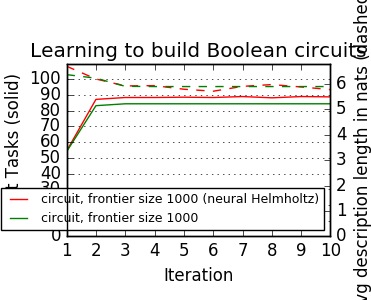
\includegraphics[width = \columnwidth]{figures/circuit.png}
  \caption{\system learning to build Boolean circuits. We start out with only NAND gates and learn DSL that contains ...}\label{circuitLearningCurve}
\end{figure}

\begin{table}
\begin{tabular}{ll}
  \toprule
  Primitives&\texttt{nand}
  
\\\midrule
  Observation $x$& $N$ input/output examples: $\left\{(i_n,o_n) \right\}_{n\leq N}$\\
  \midrule
  Likelihood $\probability[x|p]$& $\prod_n \indicator[p(i_n) = o_n]$
  \\\midrule
  \begin{tabular}{l}
    Subset of \\Learned DSL
    \end{tabular}&

  \\\bottomrule
\end{tabular}
\caption{}\label{circuitExperimentTable}
\end{table}

\subsection{Symbolic Regression}\label{regressionSection}
We show how to use \system to infer programs containing both discrete
structure and continuous parameters. The high-level idea is to synthesize programs with unspecified-real-valued parameters, and to fit those parameters using gradient descent.
Concretely, we ask the algorithm to
solve a set of 1000 symbolic regression problems, each a polynomial of
degree 0, 1, or 2, where our observations $x$ take the form of $N$
input/output examples, which we write as $x = \left\{(i_n,o_n)
\right\}_{n\leq N}$. For example, one task is to infer a program
calculating $3x + 2$, and the observations are the input-output
examples $\left\{(-1,-1),(0,2),(1,5) \right\}$.

We initially equip our DSL learner with addition and multiplication,
along with the possibility of introducing real-valued parameters, which we write as $\mathcal{R}$.
We define the likelihood of an observation $x$ by assuming a Gaussian noise model for the input/output examples and integrate over the real-valued parameters, which we collectively write as $\vec{\mathcal{R}}$:
\begin{align*}
\log   \probability\left[\{(i_n,o_n)\}|p\right] = \log \int \mathrm{d}\vec{\mathcal{R}}\; P_{\vec{\mathcal{R}}}(\vec{\mathcal{R}})\prod_{n\leq N}\mathcal{N}(p(i_n,\vec{\mathcal{R}})|o_n)
%\text{\emph{BIC:}} &\approx 
\end{align*}
where $\mathcal{N}(\cdot |\cdot )$ is the normal density  and $P_{\vec{\mathcal{R}}}(\cdot )$ is a prior over $\vec{\mathcal{R}}$. We approximate this marginal using the BIC~\cite{Bishop:2006:PRM:1162264}:
\begin{align*}
  \log \probability[x|p]  \approx& \sum_{n\leq N}\log \mathcal{N}(p(i_n,\vec{\mathcal{R}}^*)|o_n) - \frac{D\log N}{2}
\end{align*}
where $\vec{\mathcal{R}}^*$ is an assignment to $\vec{\mathcal{R}}$ found by performing gradient ascent on the likelihood of the observations w.r.t. $\vec{\mathcal{R}}$.

What DSL does \system learn?
The learned DSL contains templates for quadratic and linear functions,
which lets the algorithm quickly hone in on the kinds of functions that are most appropriate to this domain.
Examining the programs themselves,
one finds that the algorithm discovers representations for each of the polynomials that minimizes the number of continuous degrees of freedom:
for example, it represents the polynomial $8x^2+8x$

\begin{tabular}{ll}
  \toprule
  Primitives& $+,\times:\mathbb{R}\to \mathbb{R}\to \mathbb{R}$\\
  & $\mathcal{R}:\mathbb{R}$ (real valued parameter)\\\midrule
  Observation $x$& $N$ input/output examples: $\left\{(i_n,o_n) \right\}_{n\leq N}$\\
  \midrule
  Likelihood $\probability[x|p]$& $\propto\exp\left( - D\log N \right)\prod_{n\leq N}\mathcal{N}(p(i_n)|o_n)$
  \\\midrule
  \begin{tabular}{l}
    Subset of \\Learned DSL
    \end{tabular}&
  \begin{tabular}{ll}
    $\lambda x. \mathcal{R}\times x + \mathcal{R}$ &linear\\
    $\lambda x. \mathcal{R} + x$ &increment\\
    $\lambda x. x\times (\text{linear } x)$&$\text{quadratic}_0$\\
    $\lambda x. \text{increment }(\text{quadratic}_0\; x)$&quadratic\\
  \end{tabular}
  \\\bottomrule
  \end{tabular}

\begin{figure}
      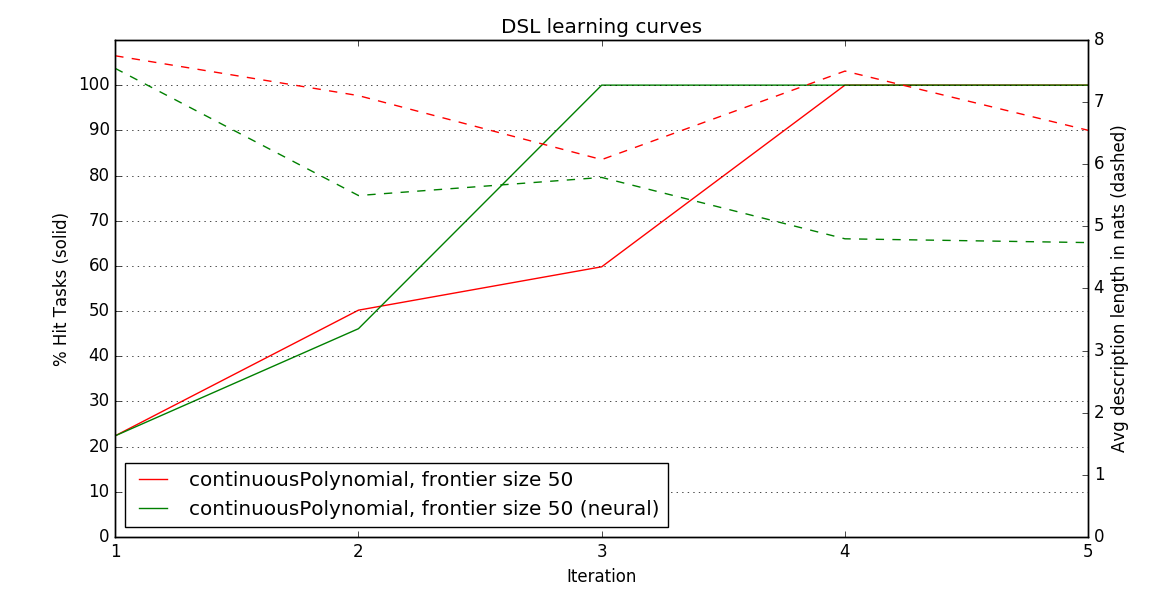
\includegraphics[width = 9cm]{figures/polynomial.png}
\end{figure}
\subsection{String editing}\label{textSection}

\begin{tabular}{ll}
  \toprule
  Primitives&\begin{tabular}{l}
    \texttt{0}, \texttt{+1},\texttt{-1}\\
    \texttt{split}, \texttt{join}, \texttt{map}, \texttt{length}, \texttt{slice}\\
    \texttt{append}, \texttt{chr->str}\\
    \texttt{lowercase}, \texttt{uppercase}, \texttt{capitalize}\\
    \texttt{""},    \texttt{","},     \texttt{" "},    \texttt{"<"}, \texttt{">"}
    \end{tabular}
  
\\\midrule
  Observation $x$& $N$ input/output examples: $\left\{(i_n,o_n) \right\}_{n\leq N}$\\
  \midrule
  Likelihood $\probability[x|p]$& $\prod_n \indicator[p(i_n) = o_n]$
  \\\midrule
  \begin{tabular}{l}
    Subset of \\Learned DSL
    \end{tabular}&

  \\\bottomrule
  \end{tabular}
\begin{figure}

  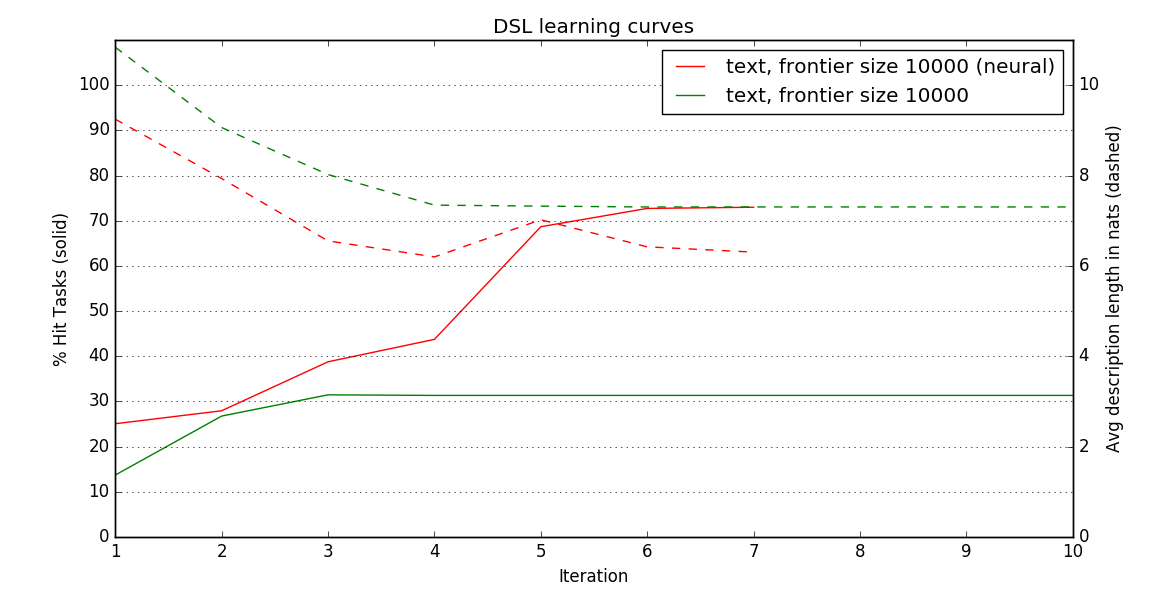
\includegraphics[width = 9cm]{figures/text.png}

\end{figure}

\subsection{List functions}
Our list function domain consists of tasks which are solved by functions
that take as input an integer or a list of integers, and have as output
either a Boolean, an integer, or a list of integers. Examples of these
functions are in Table~\ref{listexamples}. For each function, we create a
task $x$ by generating 15 input/output examples used for testing whether a
program produces the correct output. Supplying many examples reduces
ambiguity in the task's function, ensuring solutions achieve the desired
concept.

\begin{table}
\centering
\begin{tabular}{| l | l | l |}
  \hline
  \emph{name} & \emph{input} & \emph{output} \\
  \hline
  add-3 & [1\, 2\, 3\, 4] & [4\, 5\, 6\, 7] \\
  append-4 & [7\, 0\, 2] & [7\, 0\, 2\, 4] \\
  len & [3\, 5\, 12\, 1] & 4 \\
  range & 3 & [1\, 2\, 3] \\
  has-2 & [4\, 5\, 7\, 4] & \texttt{false} \\
  has-4 & [4\, 5\, 7\, 4] & \texttt{true} \\
  repeat-2 & [7\, 0] & [7\, 0\, 7\, 0] \\
  drop-3 & [0\, 3\, 8\, 6\, 4] & [6\, 4] \\
  \hline
\end{tabular}
\caption{Examples from the domain of list functions.}
\label{listexamples}
\end{table}

We supply \system with the DSL outlined in Table~\ref{listdsl}.

\begin{table}
\centering
\begin{tabular}{| l | l |}
  \hline
  \emph{name} & \emph{type} \\
  \hline
    empty & \texttt{[$\alpha$]} \\
    singleton & \texttt{$\alpha$ $\rightarrow$ [$\alpha$]} \\
    concat & \texttt{[$\alpha$] $\rightarrow$ [$\alpha$] $\rightarrow$ [$\alpha$]} \\
    map & \texttt{($\alpha$ $\rightarrow$ $\beta$) $\rightarrow$ [$\alpha$] $\rightarrow$ [$\beta$]} \\
    reduce & \texttt{($\beta$ $\rightarrow$ $\alpha$ $\rightarrow$ $\beta$) $\rightarrow$ $\beta$ $\rightarrow$ [$\alpha$] $\rightarrow$ $\beta$} \\
    \hline
    true & \texttt{bool} \\
    not & \texttt{bool $\rightarrow$ bool} \\
    and & \texttt{bool $\rightarrow$ bool $\rightarrow$ bool} \\
    or & \texttt{bool $\rightarrow$ bool $\rightarrow$ bool} \\
    \hline
    0, $\ldots$, 9 & \texttt{int} \\
    + & \texttt{int $\rightarrow$ int $\rightarrow$ int} \\
    * & \texttt{int $\rightarrow$ int $\rightarrow$ int} \\
    negate & \texttt{int $\rightarrow$ int} \\
    mod & \texttt{int $\rightarrow$ int $\rightarrow$ int} \\
    eq? & \texttt{int $\rightarrow$ int $\rightarrow$ bool} \\
    gt? & \texttt{int $\rightarrow$ int $\rightarrow$ bool} \\
    is-prime & \texttt{int $\rightarrow$ bool} \\
    is-square & \texttt{int $\rightarrow$ bool} \\
    range & \texttt{int $\rightarrow$ [int]} \\
    sort & \texttt{[int] $\rightarrow$ [int]} \\
    \hline
    sum & \texttt{[int] $\rightarrow$ int} \\
    reverse & \texttt{[$\alpha$] $\rightarrow$ [$\alpha$]} \\
    all & \texttt{($\alpha$ $\rightarrow$ bool) $\rightarrow$ [$\alpha$] $\rightarrow$ bool} \\
    any & \texttt{($\alpha$ $\rightarrow$ bool) $\rightarrow$ [$\alpha$] $\rightarrow$ bool} \\
    index & \texttt{int $\rightarrow$ [$\alpha$] $\rightarrow$ $\alpha$} \\
    filter & \texttt{($\alpha$ $\rightarrow$ bool) $\rightarrow$ [$\alpha$] $\rightarrow$ [$\alpha$]} \\
    slice & \texttt{int $\rightarrow$ int $\rightarrow$ [$\alpha$] $\rightarrow$ [$\alpha$]} \\
  \hline
\end{tabular}
\caption{DSL for the domain of list function.}
\label{listdsl}
\end{table}

\begin{figure}
  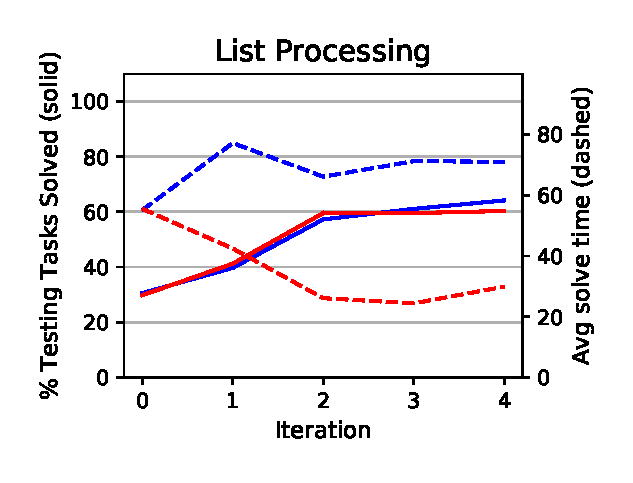
\includegraphics[width=\columnwidth]{figures/list.eps}
\end{figure}

We found that using a less sophisticated but equally-capable DSL made common
patterns, such as summation, unlikely and unlearnable in a small enumeration
bound.

\section{Model}










\bibliography{main}
\bibliographystyle{icml2018}

\end{document}


% This document was modified from the file originally made available by
% Pat Langley and Andrea Danyluk for ICML-2K. This version was created
% by Iain Murray in 2018. It was modified from a version from Dan Roy in
% 2017, which was based on a version from Lise Getoor and Tobias
% Scheffer, which was slightly modified from the 2010 version by
% Thorsten Joachims & Johannes Fuernkranz, slightly modified from the
% 2009 version by Kiri Wagstaff and Sam Roweis's 2008 version, which is
% slightly modified from Prasad Tadepalli's 2007 version which is a
% lightly changed version of the previous year's version by Andrew
% Moore, which was in turn edited from those of Kristian Kersting and
% Codrina Lauth. Alex Smola contributed to the algorithmic style files.
